% -*- latex -*-

\documentclass{article}

\usepackage{amsfonts}
\usepackage{amssymb}
\usepackage{amsmath}
\usepackage{graphicx}
\usepackage{varioref}
\usepackage{fancyvrb}
\usepackage{ifthen}
\usepackage{cite}
\usepackage{xspace}
\usepackage{hyperref}

\usepackage{color}
\definecolor{yellow}{rgb}{1,1,0}
\definecolor{black}{rgb}{0,0,0}
\definecolor{ltcyan}{rgb}{.75,1,1}
\definecolor{blue}{rgb}{0,0,1}
\definecolor{red}{rgb}{1,0,0}
\definecolor{darkred}{rgb}{0.5,0,0}
\definecolor{darkgreen}{rgb}{0,0.5,0}

% Cite commands I use to abstract away the different ways to reference an
% entry in the bibliography (superscripts, numbers, dates, or author
% abbreviations).  \scite is a short cite that is used immediately after
% when the authors are mentioned.  \lcite is a full citation that is used
% anywhere.  Both should be used right next to the text being cited without
% any spacing.
\newcommand*{\lcite}[1]{~\cite{#1}}
\newcommand*{\scite}[1]{~\cite{#1}}

\newcommand*{\keyterm}[1]{\emph{#1}}

\newcommand{\etal}{et al.}

\newcommand{\fix}[1]{{\color{red}\textbf{\textsc{[#1]}}}}

% Avoid putting figures on their own page.
\renewcommand{\textfraction}{0.05}
\renewcommand{\topfraction}{0.95}
\renewcommand{\bottomfraction}{0.5}

% Make sure this is big enough so that only big figures end up on their own
% page but small enough so that if a figure does have to be on its own
% page, it won't push everything to the bottom because it's not big enough
% to have its own page.
\renewcommand{\floatpagefraction}{.75}

\title{Modern Visualization Pipelines}

\author{Kenneth Moreland}

\date{}

\sloppy

\begin{document}

\maketitle


\section*{Abstract}

The most common abstraction used by visualization libraries and
applications today is what is known as the visualization pipeline.  The
visualization pipeline provides a mechanism to encapsulate algorithms and
then couple them together in a variety of ways.  The visualization pipeline
has been in existence for over twenty years, and over this time many
variations and improvements have been proposed.  This paper provides a
literature review of the most prevalent features of visualization pipelines
and some of the most recent research directions.


\section{Introduction}
\label{sec:Introduction}

The field of scientific visualization was launched with the 1987 National
Science Foundation Visualization in Scientific Computing workshop
report\lcite{ViSC1987}, and some of the first proposed frameworks used a
\keyterm{visualization pipeline} for managing the ingestion,
transformation, display, and recording of
data\lcite{Haeberli1988,Lucas1992}.  The combination of simplicity and
power makes the visualization pipeline still the most prevalent metaphor
encountered today.

The visualization pipeline provides the key
structure in many visualization development systems such as the
Visualization Toolkit (VTK)\lcite{VTK}, SCIRun\lcite{SCIRun}, the
Application Visualization System (AVS)\lcite{AVS}, OpenDX\lcite{OpenDX},
and Iris Explorer\lcite{IRISExplorer}.  Visualization applications like
ParaView\lcite{ParaView}, VisTrails\lcite{VisTrails}, and
MayaVi\lcite{MayaVi} allow end users to build visualization pipelines with
graphical user interface representations.  The visualization pipeline is
also used internally in a number of other applications including
VisIt\lcite{VisIt}, VolView\lcite{VolView}, OsiriX\lcite{OsiriX}, 3D
Slicer\lcite{3DSlicer}, and BioImageXD\lcite{BioImageXD}.

In this paper we review the visualization pipeline.  We begin with a basic
description of what the visualization pipeline is and then move to
advancements introduced over the years and current research.


\section{Basic Visualization Pipelines}
\label{sec:BasicVisualizationPipelines}

A visualization pipeline encapsulates an algorithm in one of three types of
objects: \keyterm{sources}, \keyterm{filters}, and \keyterm{sinks}.  A
source object produces data that it makes available through an
\keyterm{output}.  File readers and synthetic data generators are typical
source objects.  A sink object accepts data through an \keyterm{input} and
performs an operation with no further result (as far as the pipeline is
concerned).  Typical sinks are file writers and rendering components that
provide images to a user interface.  A filter object has at least one input
from which it transform data and provides results through at least one
output.

The intention is to encapsulate algorithms in interchangeable source,
filter, and sink components with generic connection ports (inputs and
outputs).  An output from one component can be connected to the input from
another component such that the results of one algorithm become the inputs
to another algorithm.  These connected components form a
\keyterm{pipeline}.  Figure~\ref{fig:SimplePipeline} demonstrates a simple
but common pipeline featuring a file reader (source), an isosurface
generator\lcite{Lorensen1987} (filter), and an image renderer (sink).

\begin{figure}[htbp]
  \centering
  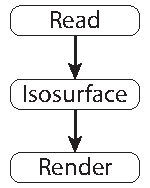
\includegraphics{images/SimplePipeline}
  \caption{A simple visualization pipeline.}
  \label{fig:SimplePipeline}
\end{figure}

Pipeline components are highly interchangeable.  Any two components can be
connected so long as the data in the output is compatible with the expected
data of the downstream input.  Pipelines can be arbitrarily deep.
Pipelines can also branch.  A \keyterm{fan out} occurs when the output of
one component is connected to the inputs of multiple other components.  A
\keyterm{fan in} occurs when a component accepts multiple inputs that can
come from separate component outputs.  Figure~\ref{fig:BranchingPipeline}
demonstrates a pipeline with branching (adapted from the ParaView
tutorial\lcite{ParaViewTutorial}).

\begin{figure}[htbp]
  \centering
  \begin{tabular}{cc}
    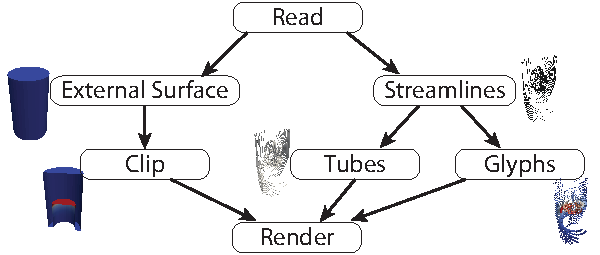
\includegraphics{images/BranchingPipeline} &
    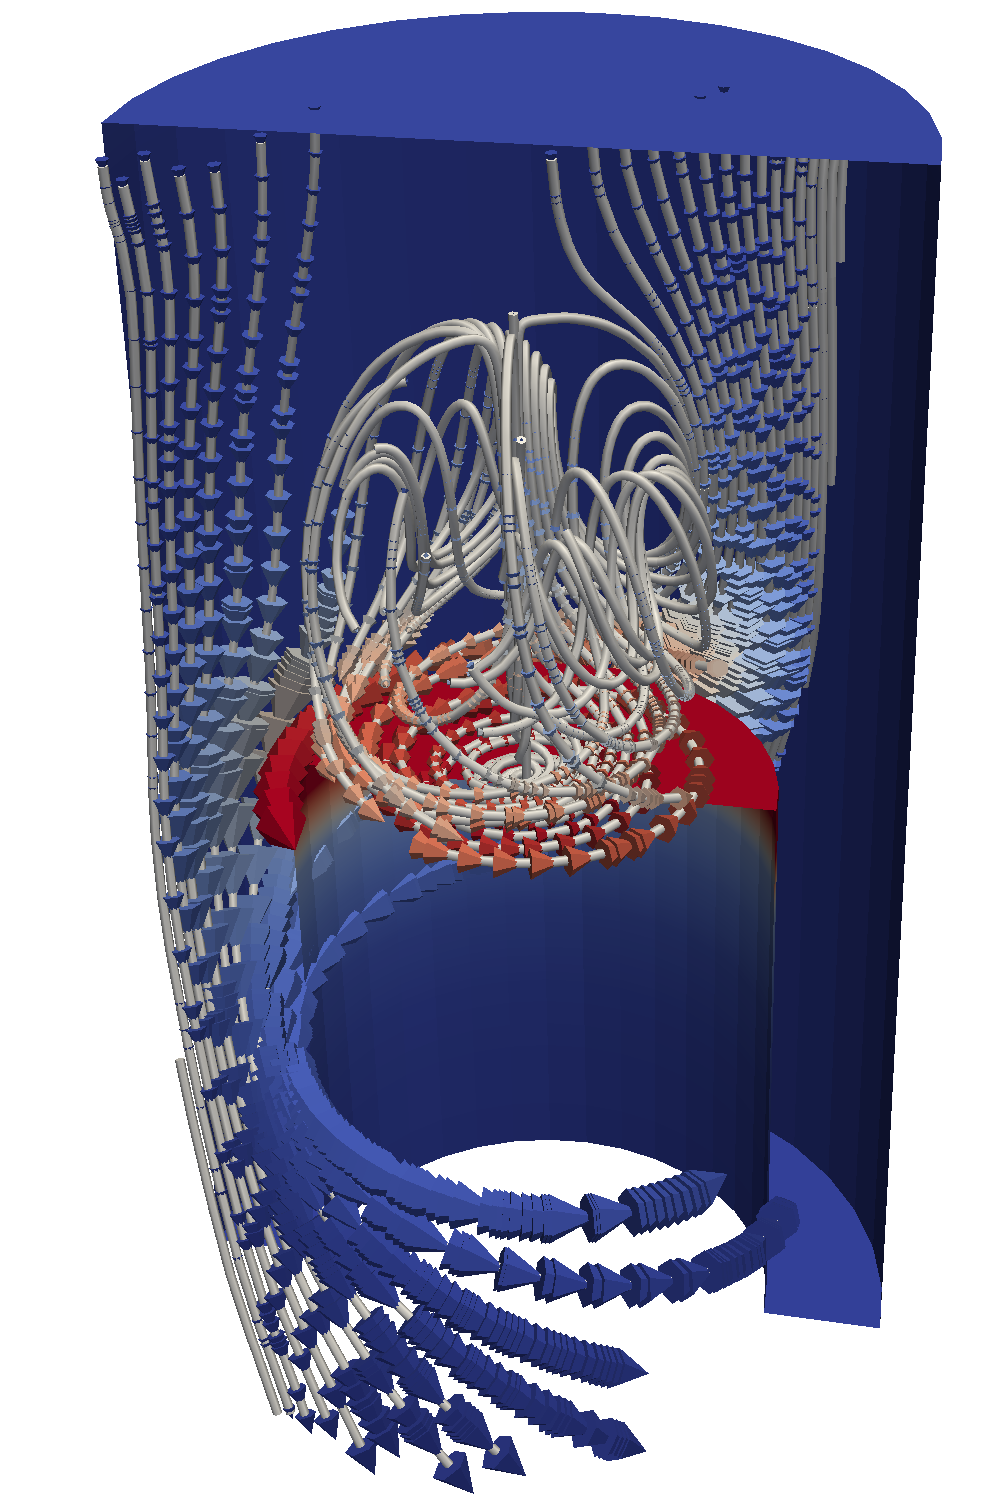
\includegraphics[height=1.7in]{images/BranchingPipelineResult}
  \end{tabular}
  \caption{A visualization pipeline with branching.  The final
    visualization is shown to the right.}
  \label{fig:BranchingPipeline}
\end{figure}

For more information on using visualization pipelines and the components
they typically contain, consult the documentation for one of the numerous
libraries or applications using a visualization
pipeline\lcite{VTK,ParaView,ParaViewTutorial,SCIRunUserGuide,IRISExplorerUsersGuide,VisTrailsDocumentation}.
\fix{Add OpenDX.  Site was down.}


\section{Execution Management}
\label{sec:ExecutionManagement}

The topology of a pipeline dictates the flow of data and places constraints
on the order in which components can be executed, but it does not determine
how or when components get executed.  Visualization pipeline systems can
vary significantly in how they manage execution.

\subsection{Execution Drivers}
\label{sec:ExecutionDrivers}

The visualization pipeline represents a static network of operations
through which data flows.  Typical usage entails first establishing the
visualization pipeline and then executing the pipeline on one or more data
collections.  Consequently, the behavior of when components get executed is
a primary feature of visualization pipeline systems.  Visualization
pipelines generally fall under two execution systems: event driven and
demand driven.

An \keyterm{even-driven} pipeline launches execution as data becomes
available in sources.  When new data becomes available in a source, that
source component must be alerted.  When sources produce data, they push it
to the downstream components and trigger an event to execute them.  Those
downstream components in turn may produce their own data to push to the
next component.  Because the method of the event-driven pipeline is to push
data to the downstream components, this method is also known as the
\keyterm{push model}.  The event-driven method of execution is useful when
applying a visualization pipeline to data that is expected to change over
time.

A \keyterm{demand-driven} pipeline launches execution in response to
requests for data.  Execution is initiated at the bottom of the pipeline in
a sink.  The sink's upstream components satisfy this request by first
requesting data from their upstream components, and so on up to the
sources.  Once execution reaches a source, it produces data and returns
execution back to its downstream components.  The execution eventually
unrolls back to the originating sink.  Because the method of the
demand-driven pipeline is to pull data from the upstream components, this
method is also known as the \keyterm{pull model}.  The demand-driven method
of execution is useful when using a visualization pipeline to provide data
to an end system.  For example, the visualization could respond to render
requests to update a GUI.

\subsection{Caching Intermediate Values}
\label{sec:Caching}

Caching, which saves component execution outputs, is an important feature
for both execution methods.  In the case of the event-driven pipeline, a
component may execute only when data from all inputs is pushed to it.
Thus, the execution must know when to cache the data and where to retrieve
it when the rest of the data is later pushed.

In the case of the demand-driven pipeline, a component with fan out could
receive pull requests from multiple downstream components during the same
original sink request.  Rather than execute multiple times, the component
can first check to see if the previously computed result is still valid and
return that if possible.

Although caching all the intermediate values in a pipeline can remove
redundant computation, it also clearly requires more storage.  Thus,
managing the caching often involves a trade-off between speed and memory.
The cost of caching can be mitigated by favoring shallow copies of data
from a component's inputs to its outputs.

\subsection{Centralized vs. Distributed Control}
\label{sec:CentralizedDistributed}

The control mechanism for a visualization pipeline can be either
centralized or distributed.  A \keyterm{centralized control} has a single
unit managing the execution of all components in the pipeline.  The
centralized control has links to all components, understands their
connections, and initiates all execution in the pipeline.

A \keyterm{distributed control} has a separate unit for each component in
the pipeline.  The distributed control unit nominally knows only about a
single component and its inputs and outputs.  The distributed control unit
can initiate execution on only its own component and must send messages to
propagate execution elsewhere.

Centralized control is advantageous in that it can perform a more
thorough analysis of the pipeline's network to more finely control the
execution.  Such knowledge can be useful in making decisions about caching
(described in Section~\ref{sec:Caching}) and load balancing for parallel
execution (described in Section~\ref{sec:ParallelExecution}).  However, the
implementation of a centralized control is more complex because of the
larger management task.  Distributed control, in contrast, has more limited
knowledge of the pipeline, but tends to be simpler to implement and
manage.

\subsection{Interchangeable Executive}
\label{sec:InterchangeableExecutive}

Many visualization pipeline implementations have a fixed execution
management system.  However, such a system can provide more flexibility by
separating its execution management into a \keyterm{executive} object.  The
executive object is an independent object that manages pipeline execution.
Through polymorphism, different types of execution models can be
supported.  For example, VTK is designed as a demand-driven pipeline, but
with its interchangeable executives it can be converted to an event-driven
pipeline, as demonstrated by Vo \etal\lcite{Vo2010}.

Replacing the executive in a pipeline with centralized control is
straightforward.  The control is, by definition, its own separate unit.  In
contrast, a distributed control system must have an independent executive
object attached to each component in the pipeline.  The component objects
get relegated to only a function to execute whereas the executive manages
pipeline connections, data movement, and execution\lcite{VTKUsersGuide}.

\subsection{Block Iteration}
\label{sec:BlockIteration}

Some data sets are actually a conglomerate of smaller data sets.  These
smaller data sets are called either \keyterm{blocks} or \keyterm{domains}
of the whole.  One example of a multi-block data set is an assembly of
parts.  Another example is adaptive mesh refinement (AMR)\lcite{Berger1989}
in which a hierarchy of progressively finer grids selectively refines
regions of interest.

Many visualization algorithms can be applied independently to each block in
a multi-block data set.  Rather than have every component specifically
attend to the multi-block nature of the data, the execution management can
implicitly run an algorithm independently on every block in the data
set\lcite{VTKUsersGuide}.


\section{Metadata}
\label{sec:Metadata}

\subsection{Regions}
\label{sec:Regions}

Types of regions: extents, pieces, blocks/domains.

Ghost cells.

Reporting regions in multiple passes.

Sending region requests up pipeline.

\subsection{Contracts}
\label{sec:Contracts}

\subsection{Time}
\label{sec:Time}

\subsection{Prioritized Streaming}
\label{sec:PrioritizedStreaming}

\subsection{Query Driven Visualization}
\label{sec:QueryDrivenVisualization}


\section{Parallel Execution}
\label{sec:ParallelExecution}

\subsection{Basic Parallel Execution Modes}
\label{sec:ParallelExecution:Modes}

\subsection{Rendering}
\label{sec:ParallelExecution:Rendering}

\subsection{Scalability}
\label{sec:Scalability}

\subsection{Hybrid Parallel}
\label{sec:HybridParallel}


\section{Miscellany}
\label{sec:Misc}

\subsection{Provenance}
\label{sec:Provenance}

\subsection{Scheduling}
\label{sec:Scheduling}

Multi-core.  Heterogeneous.  Hyperflow.

\subsection{In Situ}
\label{sec:InSitu}


\section{Visualization Pipeline Alternatives}
\label{sec:Alternatives}

\subsection{Field Abstraction}
\label{sec:FieldAbstraction}

Field Model (FM).  Field Encapsulation Library (FEL).

\subsection{MapReduce}
\label{sec:MapReduce}

\subsection{Worklets}
\label{sec:Worklets}


\section{Conclusion}
\label{sec:Conclusion}


\section{Acknowledgments}

This work was supported in part by the DOE Office of Science, Advanced
Scientific Computing Research, under award number 10-014707, program
manager Lucy Nowell.

Sandia National Laboratories is a multi-program laboratory operated by
Sandia Corporation, a wholly owned subsidiary of Lockheed Martin
Corporation, for the U.S. Department of Energy's National Nuclear Security
Administration.

\bibliographystyle{plain}
\bibliography{VisPipelines}

\end{document}
